\chapter{Unseen Quantum State Generation}
\label{chapter:my_contribution}
In the previous chapter we evaluated two different types of quantum GANs. The
common problem of those is the inability to generate new, unseen states. In this
chapter we propose the hybrid classical-quantum framework that can overcome this limitation. 

Our idea is based WQGANs and how the quantum Wasserstein distance is
approximated during the training. The discriminator at every step approximates
the distance between some fixed, real input state and the generated state which
changes after each iteration. However, the discriminator never needs an access to
the actual real input state, it only operates on the set of measured
expectations. 

Given a parametrized circuits $U$
and set of parameters $\Theta = \{\theta_i\}$ and a set of operators $H =
\{H_j\}$, we prepare a set of vectors of expectations $S$. Each vector $s_{\theta_i}
\in S$ contains the expectations of the circuit $U(\theta_i)$, such that
$s_{\theta_i}^{(j)} = \langle H_j \rangle_{U(\theta_i)} $.

Assuming that all the vectors in $S$ come from the same distribution $p_S$,
the proposed framework is defined in two parts as follows:
\begin{enumerate}
\item \textit{Classical}: Takes as the input the set $S$ and uses it to learn a function $f:
  \mathbb{R}^{n} \to \mathbb{R}^{|H|}$. Given an arbitrary vector $g \in
  \mathbb{R}^n$ (e.g. random noise), this function produces a new vector $s' =
  f(g)$ such that $s' \sim p_S$.  
\item \textit{Quantum}: Takes $s'$ as the input and uses it as
  expectations of real input source in the WQGANs setting described in the
  previous chapter. The generator trained using $s'$ produces new, unseen before
  quantum state. The WQGANs optimization objective from Equation
  \ref{eq:wqgans_optimization_objective} becomes:
  \begin{equation}
    \max_{w}{\min_{\theta}{\mathcal{L}(w, \theta)}} = \max_{w}{\min_{\theta}{(\sum_{i=1}^Nw_i(s^{\prime(i)} - Tr[G(\theta)H_i]))}} 
    \label{eq:wqgans_optimization_objective_unseen}
  \end{equation}
\end{enumerate}

Once the function $f$ is learnt, it can be used arbitrary many times to produce
new vectors of expectations.
With those vectors, it is possible to generate new quantum states that come from
some circuit $U(\theta')$, without ever knowing $U$ or $\theta'$.
In the following sections, we show how exactly the function $f$ can be obtained
for two different cases. 
\section{Labeled State Generation}
If the quantum state produced by the circuit $U$ can be labeled by some continuous
variable, we can use this variable to find the function $f$.

Specifically, here we assume that each parameter $\theta_i^{(j)}$ is described by some
function, i.e. $\theta_i = \theta(g_i) = [\theta^{(1)}(g_i), \theta^{(2)}(g_i), \ldots,
\theta^{(l)}(g_i)]$, for some $g_i \in V \subseteq 
\mathbb{R}$, where $l$ is the number of parameters in the circuit $U$.
We also assume that the expectations of the state produced by the
circuit $U(\theta(g_i))$, can be described by some other functions,
i.e. $s_{\theta_i} = s(g_i) = [s^{(1)}(g_i), s^{(2)}(g_i), \ldots,
s^{(|H|)}(g_i)]$, $s^{(j)}: V \to [-1; 1]\ \forall_{j \in 1,\ldots,|H|}$.
Then, the input to the classical part of the framework is the set $S$, together with
corresponding $g_i$ for each $s_{\theta_i} = s(g_i) \in S$.
To find $s^{(j)}\ \forall_{j=1,\ldots,|H|}$ functions interpolation is
sufficient. So, the function $f: V \to \mathbb{R}^{|H|}$ simply takes
any value of $g \in V$ and returns the expectations for this value using
interpolations of functions $s^{(j)}$.

\subsection{Evaluation Results}
This approach can be used when $U$ is the topological phase transition circuit from
Appendix \ref{apx:topological_phase_transition_ansatz}. All the parameters of
this circuit can be described by three functions $\theta_v, \theta_w, \theta_r$
over $V = [-1; 1]$. To prepare the input to the classical part 
 $m$ ($m = |S|$) values of $g \in V$ are sampled and the expectations of $U(\theta_v(g_i),
\theta_w(g_i), \theta_r(g_i))\ \forall_{i=1,\ldots,m}$ are calculated for all operators $H_i
\in H$. Similarly as in the WQGANs chapter, $H$ is chosen to be a
set of all k-length Pauli Strings.
This data is used to interpolate the expectation functions for those operators.  

In Figure \ref{fig:phase_exps} interpolated expectations of the circuit for
$k=3$ and $m=11$ are plotted (only subset of the expectation is plotted for readability).

\begin{figure}[htbp!]
  \captionsetup[subfigure]{labelformat=empty}
  \centering
  \subfloat{
    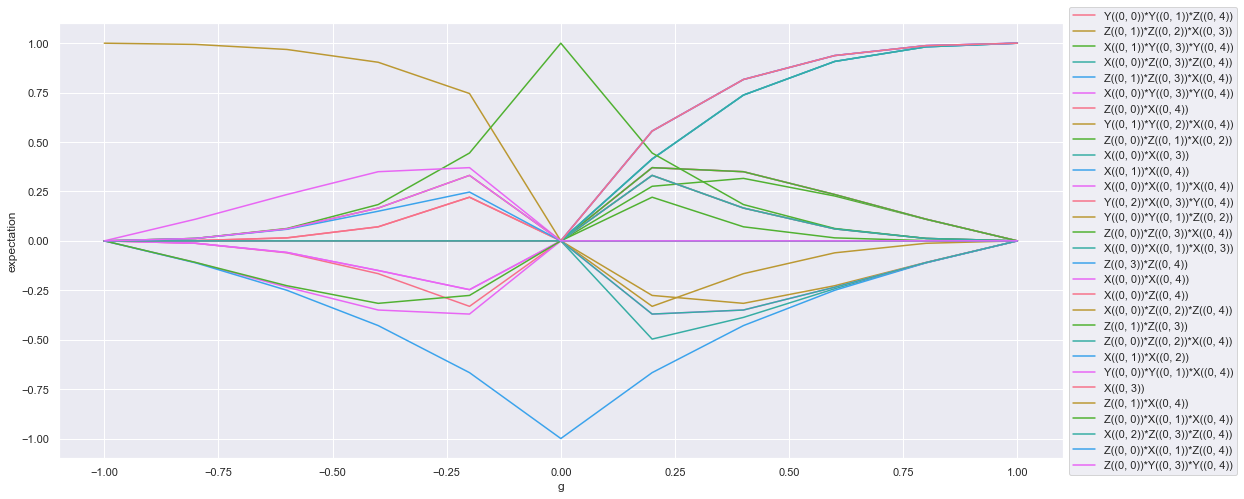
\includegraphics[width=1\linewidth]{figures/phase_exps/plot.png}
  }
  \caption{Interpolated expectations of topological phase transition circuit (Appendix
    \ref{apx:topological_phase_transition_ansatz}) with 5 qubits width for 30
    random 3-Pauli Strings operators. Interpolation using evenly
    spaced 11 values of the parameter $g \in [-1; 1]$. 
  }
  \label{fig:phase_exps}
\end{figure}

The interpolated expectations are used to learn the quantum states for
the values of $g$ that were not part of the classical input. In Figure
\ref{fig:wqgans_res_interpolated_1} we see fidelity and Wasserstein distance
between the real input states and the ones learnt using the interpolated
expectations.
Those results are comparable with the ones obtained by learning from known
expectations (Figure \ref{fig:wqgans_res_1}).

\begin{figure}[htbp!]
  \captionsetup[subfigure]{labelformat=empty}
  \centering
  \subfloat{
    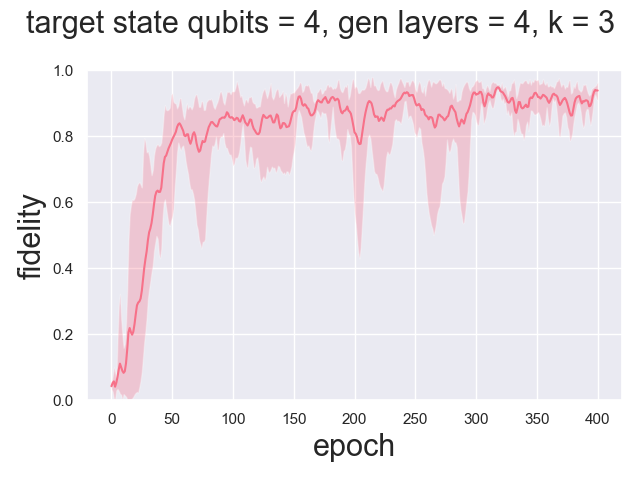
\includegraphics[width=0.25\linewidth]{figures/wqgans_phase_size=4_k=3_gen=4_interpolation/fidelity.png}
  }
  \subfloat{
    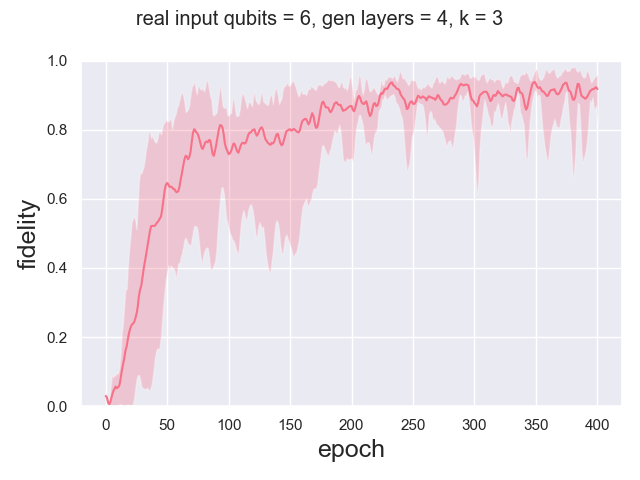
\includegraphics[width=0.25\linewidth]{figures/wqgans_phase_size=6_k=3_gen=4_interpolation/fidelity.png}
  }
  \subfloat{
    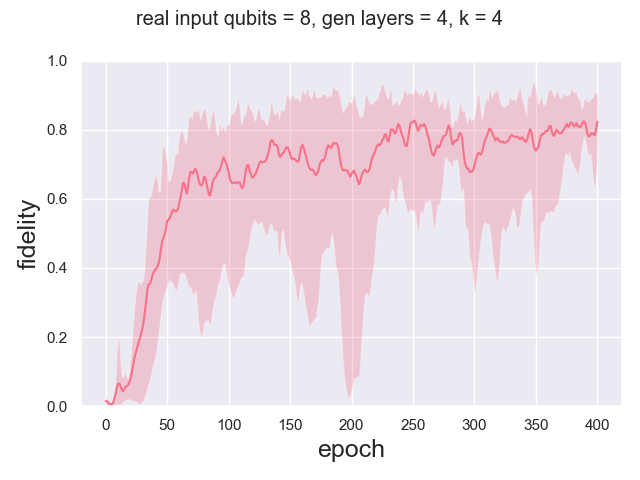
\includegraphics[width=0.25\linewidth]{figures/wqgans_phase_size=8_k=4_gen=4_interpolation/fidelity.png}
  }
  \subfloat{
    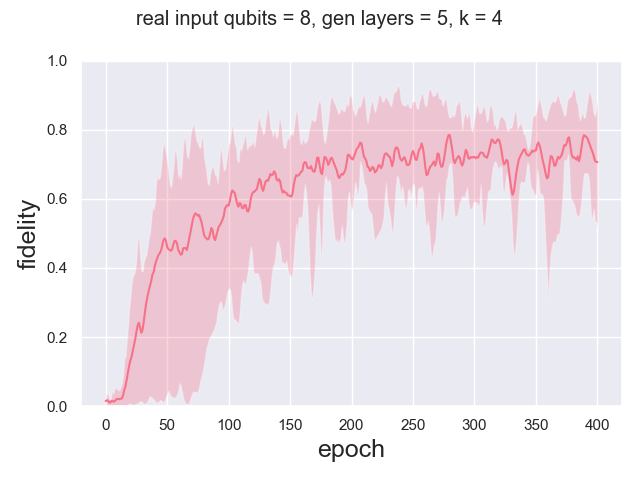
\includegraphics[width=0.25\linewidth]{figures/wqgans_phase_size=8_k=4_gen=5_interpolation/fidelity.png}
  }

  \subfloat{
    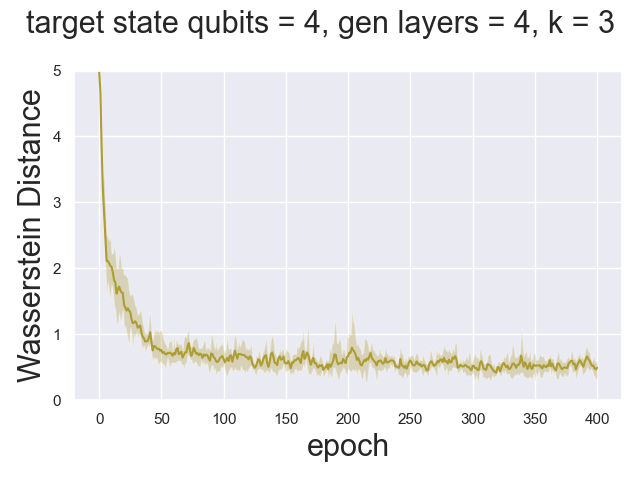
\includegraphics[width=0.25\linewidth]{figures/wqgans_phase_size=4_k=3_gen=4_interpolation/Wasserstein_Distance.png}
  }
  \subfloat{
    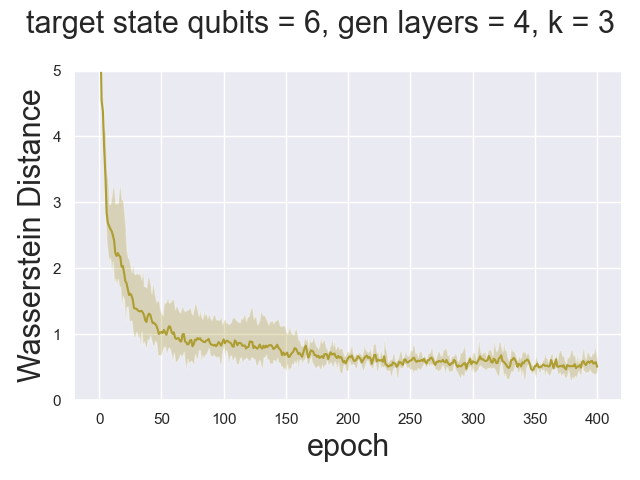
\includegraphics[width=0.25\linewidth]{figures/wqgans_phase_size=6_k=3_gen=4_interpolation/Wasserstein_Distance.png}
  }
  \subfloat{
    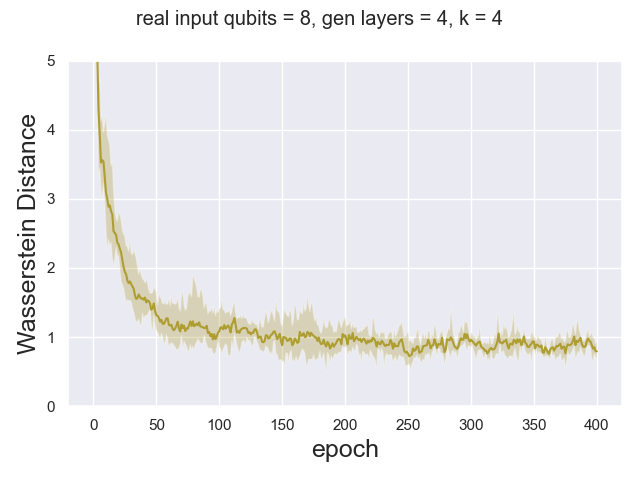
\includegraphics[width=0.25\linewidth]{figures/wqgans_phase_size=8_k=4_gen=4_interpolation/Wasserstein_Distance.png}
  }
  \subfloat{
    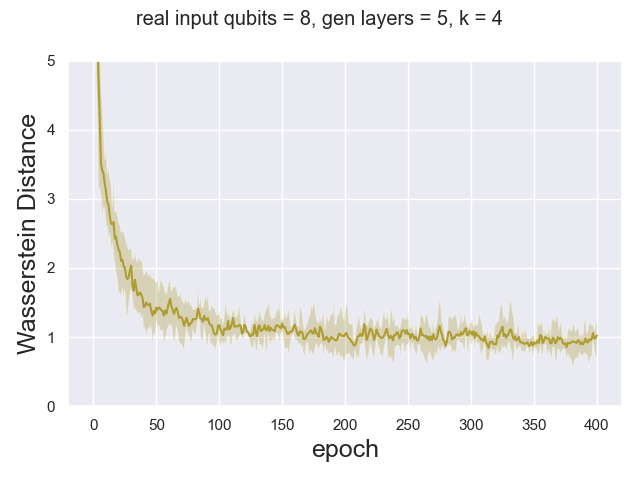
\includegraphics[width=0.25\linewidth]{figures/wqgans_phase_size=8_k=4_gen=5_interpolation/Wasserstein_Distance.png}
  }
  \caption{Results for topological phase transition circuit (ansatz Appendix
    \ref{apx:topological_phase_transition_ansatz}) using interpolated expectations.
    The solid line represents the average value and the shaded area
    represents the range from 5 different experiments. The upper row shows the
    fidelity and the bottom row shows the corresponding Wasserstein distance. In all the
    experiments the generator is built using ansatz from Appendix
    \ref{apx:sqgans_ansatz}. }
  \label{fig:wqgans_res_interpolated_1}
\end{figure}

\subsubsection{String Order Parameters}

In their work Smith et. al\cite{smith2020crossing} define two
string order parameters
\begin{equation}
\begin{split}
S^\mathbb{1} =  & \bra{\psi}(\prod_{i=3}^{N-2}X_i)\ket{\psi} \\
S^{ZY} =  & \bra{\psi}Z_2Y_3(\prod_{i=4}^{N-3}X_i)Y_{N-2}Z_{N-1}\ket{\psi},
\end{split}
\end{equation}
where $N$ is the width of the circuit and $\ket{\psi}$ is the final state
obtained by the topological phase transition circuit from Appendix
\ref{apx:topological_phase_transition_ansatz}.
The measurements of $S^{\mathbb{1}}$ and $S^{ZY}$ on states learnt using the
interpolated expectations are shown in Figure \ref{fig:string_order_1}. The
obtained results closely follow the expected value and the phase transition
point at $g=0$ is clearly distinguishable.

\begin{figure}[htbp!]
  \captionsetup[subfigure]{labelformat=empty}
  \centering
  \subfloat{
    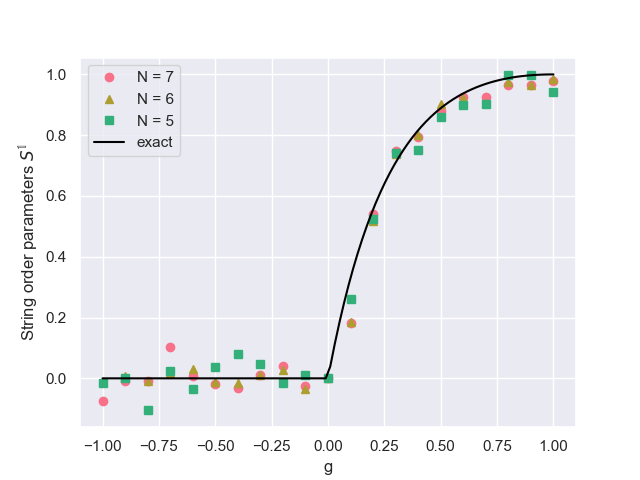
\includegraphics[width=0.5\linewidth]{figures/string_order_s1/plot.png}
  }
  \subfloat{
    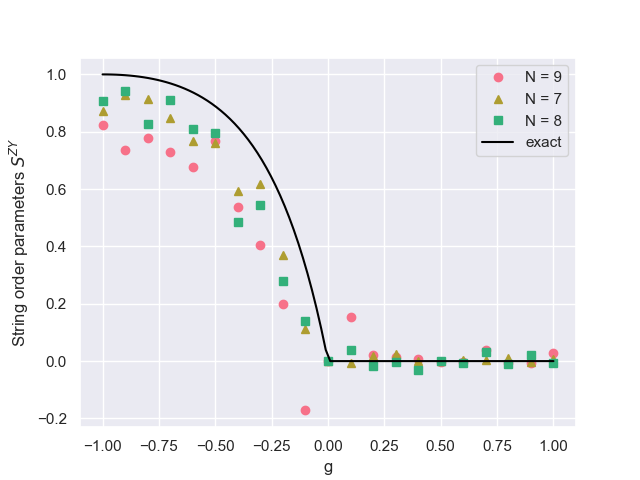
\includegraphics[width=0.5\linewidth]{figures/string_order_szy/plot.png}
  }
  \caption{String order parameters $S^\mathbb{1}$ and $S^{ZY}$ measured on the
    generic generator from Appendix \ref{apx:sqgans_ansatz}, trained using the
    interpolated expectations, for different width of circuit $N$.
    The phase transition at $g=0$ is clearly visible,
    the results are very close to the exact ones.}
\label{fig:string_order_1}
\end{figure}

\subsection{Conclusions}
Using the interpolated expectations allows to learn unknown quantum states.
In all the experiments generic generator ansatz was used, meaning that also the
design of $U$ its parametrization was unknown to the quantum Generator and
Discriminator.

Although the setup described here assumes one dimensional variable $g$, this
notion can be extended to multi-variable case where $g \in V \subseteq
\mathbb{R}^m$.



\section{Unlabeled State Generation}
In the general case the assumptions from the previous Section do not hold and
more powerful tools are need to find the function $f$. However, following the assumption
that all vectors in input set $S$ come from the same distribution $p_S$, we can use
the generative modeling to learn the function $f$. In particular, here we use
classical Wasserstein Generative Adversarial Networks (WGANs) to approximate the
distribution $p_S$ and later use the classical Generator as the function $f$ to
produce the vectors $s'$. 

\subsection{Evaluation Results}
We use this technique to generate new, previously unseen states from the butterfly circuit
(Appendix \ref{apx:butterfly_ansatz}). First we generate the set $S$ and use it
to train a simple WGAN with gradient penalty\cite{gulrajani2017improved}, with
penalty factor $10$. We use
simple 2-layers deep neural network for both, generator and discriminator and Adam
optimizer \cite{kingma2017adam} with the following parameters $\beta_1 = 0$,
$\beta_2 = 0.9$, $\hat{\epsilon} = 1e - 9$ and learning rate of $0.0001$. The layers
dimensions of generator and discriminator varies depending on the real input width 
and are specified separately.

%%% Local Variables:
%%% mode: latex
%%% TeX-master: "../main"
%%% End: